% TU Delft beamer template
% Author: Erwin Walraven (initial version was created by Maarten Abbink)
% Delft Universiy of Technology

\documentclass{beamer}
\usepackage{amsmath}
\usepackage{amsfonts}
\usepackage{amsthm}
\usepackage{mathtools}
\usepackage[english]{babel}
\usepackage{calc}
\usepackage[absolute,overlay]{textpos}
\usepackage{graphicx}
\usepackage{subfig}
\usepackage{comment}
%\usepackage{tikz}
\usepackage{wasysym}
\usepackage{gensymb}
\usepackage{amssymb}
\usepackage{nccmath}
\usepackage{empheq}
\usepackage{xcolor}
\usepackage{relsize}
%\usepackage{apalike}
\usepackage[utf8]{inputenc}
\usepackage{multimedia}
\usepackage{media9}
%\usepackage{hyperref}.
\usepackage[table]{colortbl}


\usepackage{arydshln}


\makeatletter
\renewcommand*\env@matrix[1][*\c@MaxMatrixCols c]{%
	\hskip -\arraycolsep
	\let\@ifnextchar\new@ifnextchar
	\array{#1}}
\makeatother


\newcommand*\widefbox[1]{\fbox{\hspace{1em}#1\hspace{1em}}}
%\useoutertheme{miniframes}

%\usefonttheme[onlymath]{serif}



\setbeamertemplate{navigation symbols}{} % remove navigation symbols
\mode<presentation>{\usetheme{tud}}


%\ExecuteBibliographyOptions{parentracker=false}



% BIB SETTINGS
%\usepackage[backend=bibtex,firstinits=true,maxnames=30,maxcitenames=20,url=false,style=authoryear]{biblatex}
%\bibliography{MyBib}
%\addbibresource{MyBib.bib}
%\setlength\bibitemsep{0.3cm} % space between entries in the reference list
%\renewcommand{\bibfont}{\normalfont\scriptsize}
%\setbeamerfont{footnote}{size=\tiny}
%\makeatletter
%\renewcommand{\cite}[1]{\footnote<.->[frame][{\fullcite{#1}}]}
%\renewcommand{\cite}[1]{$[$\cite{#1}$]$}


% Insert frame before each subsection (requires 2 latex runs)
\AtBeginSection {
	\begin{frame}<beamer>[noframenumbering] \frametitle{\titleSubsec}
		\tableofcontents[currentsection,currentsubsection]  % Generation of the Table of Contents
	\end{frame}
}

% Define the title of each inserted pre-subsection frame
\newcommand*\titleSubsec{Outline}
% Define the title of the "Table of Contents" frame
\newcommand*\titleTOC{Outline}

\graphicspath{ {./images/} } 

\title[PhD meeting: Planning and Control]{PhD meeting \vspace{15pt}}
\institute[]{Istituto Italiano di Tecnologia, Genova, Italy \vspace{20pt}}
\author{Octavio A. Villarreal Maga\~na \vspace{20pt}} %\scriptsize Committee:  \\ Prof.Dr.Ir. Nathan van de Wouw (TUDelft, supervisor) \\ \vspace{1.5pt} \hspace{-11pt}Prof.Dr.Ir. Emmanuel Detournay (UMN, supervisor) \\ \vspace{-2.5pt} \hspace{-74pt}Dr.Ir. Manuel Mazo Jr. (TUDelft)}
\date{\today}

\begin{document}
{
\setbeamertemplate{footline}{\usebeamertemplate*{minimal footline}}
\frame{\titlepage}
%\begin{frame}\frametitle{\titleTOC}
%	\tableofcontents
%\end{frame}
}

{\setbeamertemplate{footline}{\usebeamertemplate*{minimal footline}}
}



\begin{frame}{Outline}
	\begin{itemize}\setlength\itemsep{2em}
		\item Implementation of gait generation using max-plus
		\item Maintenance of HyQ and lab
		\item Summer schools 
		\item Meeting with M. Shahbazi 
		\item Further work
	\end{itemize}
\end{frame}

\begin{frame}{Implementation of gait generation using max-plus}
\begin{itemize}\setlength\itemsep{3em}
\item Created max-plus algebra class on C++
\item Created max-plus scheduler class on C++
\item Implemented code on RCF controller
\item Trotting gait ($D_f = 0.5$)
\end{itemize}
\end{frame}


\begin{frame}{Simulation}
\movie[width=\textwidth,showcontrols=true]
        {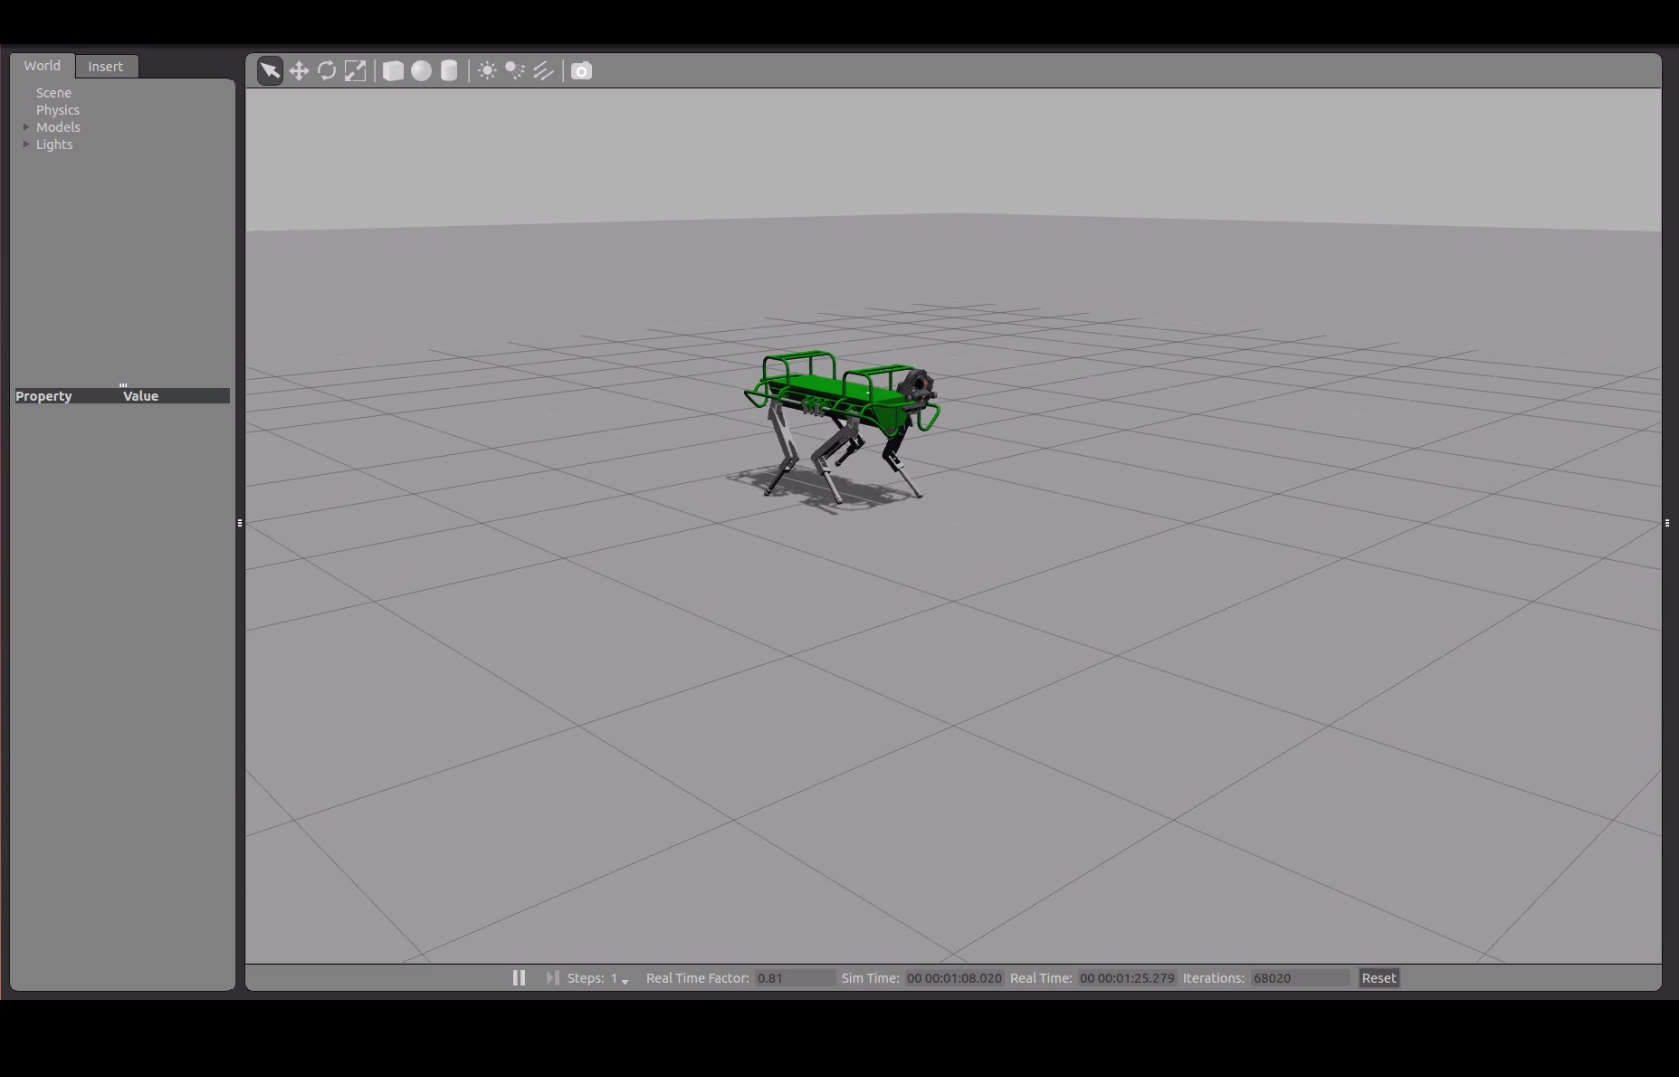
\includegraphics[width=\textwidth]{OUTPUT.png}}{OUTPUT.mp4} \\
\end{frame}

\begin{frame}{Work for the next month}
\begin{itemize}\setlength\itemsep{3em}
\item Implement "event feedback" in simulation
\item Test gait parameter switching
\item Improve code
\end{itemize}
\end{frame}

\begin{frame}{Summer schools}
\begin{itemize}
\item Machine Learning Crash Course (Genova, Italy, June 26th - 30th)
\begin{itemize}
\item Admitted (almost certain)
\item No admission fee
\end{itemize}
\item BMVA Computer Vision Summer School (Lincoln, UK, July 3rd - 7th)
\begin{itemize}
\item Registration opened (not submitted yet)
\item Non UK + accommodation: £670, no accommodation: £494
\end{itemize}
\item Numerical Optimization and Optimal Control (Rome, Italy, June 19th - 23rd)
\begin{itemize}
\item Registered (no confirmation)
\item Probably not going since it is a workshop and discussion may be not so relevant for my project
\end{itemize}
\end{itemize}
\end{frame}

\begin{frame}{Meeting with M. Shahbazi}
\begin{itemize}\setlength\itemsep{2em}
\item Former PhD student in Delft
\item Work on max-plus algebra for locomotion systems
\item Simplified double SLIP-model
\item Discussed on his perspectives to extend his work
\item On a different scope than the one of the group
\end{itemize}
\end{frame}

\begin{frame}{Further work}
	\begin{itemize}\setlength\itemsep{3em}
		\item Implement the already mentioned features to max-plus in simulation
		\item Think about generalizing the gait generation for different controllers within the group (Michele's, Carlos')
	\end{itemize}
\end{frame}

\begin{frame}
 \hspace{2cm} Thank you. Questions or comments?
\end{frame}





\end{document}
